As a comparison point for PIP's ability to manage continuous random variables, we have constructed a sample-first probabilistic extension to Postgres that emulates MCDB's tuple-bundle concept using ordinary Postgres rows.  A sampled variable is represented using an array of floats, while the tuple bundle's presence in each sampled world is represented using a densely packed array of booleans.  In lieu of an optimizer, test queries were constructed by hand so as to minimize the lifespan of either array type.

Using Postgres as a basis for both implementations places them on an equal footing with respect to DBMS optimizations unrelated to probabilistic data.  This makes it possible to focus our comparison solely on the new, probabilistic functionality of both systems.  However, to make the distinction explicit, we refer to our implementation of MCDB as Sample-First.

We evaluated both the PIP C-Tables and the Sample-First infrastructure against a variety of related queries.  Tests were run over a single connection to a modified instance of PostgreSQL 8.3.4 with default settings running on a 2x4 core 2.0 GHz Intel Xeon with a 4MB cache.  All queries were evaluated over a 1 GB database generated by the TPC-H benchmark.  Unless otherwise specified, all sampling processes generate 1000 samples apiece.  Unless otherwise specified, results shown are the average of 10 trials run sequentially.  

The first set of tests evaluate PIP's performance on queries similar to those used in \cite{MCDB}.  The results of these tests are shown in Figure \ref{fig:querytimings}.  Performance times for PIP are divided into two components: query and sample, to distinguish between time spent evaluating the deterministic components of a query and building the result c-table, and time spent computing expectations and confidences of the results.

\begin{figure}
\begin{center}
\resizebox{3in}{!}{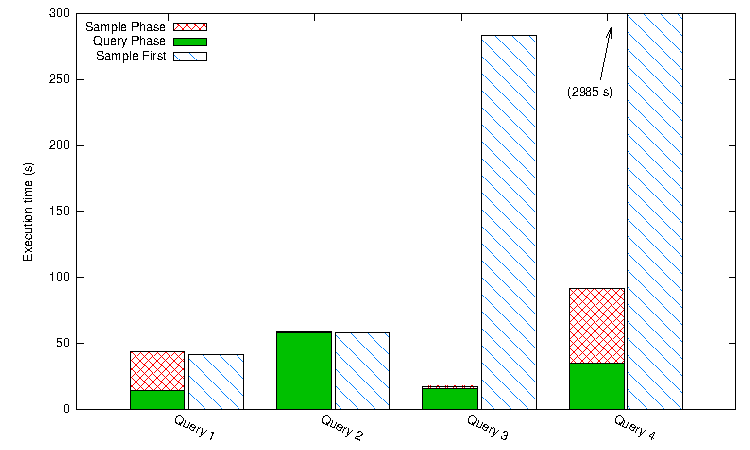
\includegraphics{graphics/query_timings.pdf}}
\caption{Query evaluation times in PIP and Sample-First: For simple aggregate queries such as Q1 and Q2, PIP and Sample-First perform comparably.  PIP and Sample-First's comparable performance on selective queries such as Q3 is misleading, as Sample-First must ignore a large number of samples and generates a less accurate result than PIP.  A simplified version of Q3 is run as Q4, where Sample-First generates a sufficient number of samples to obtain a comparable variance.}
\label{fig:querytimings}
\end{center}
\end{figure}

The first query computes the rate at which customer purchases have increased over the past two years.  The percent increase parametrizes a Poisson distribution that is used to predict how much more each customer will purchase in the coming year.  Given this predicted increase in purchasing, the query estimates the company's increased revenue for the coming year.

In the second and third queries, past orders are used to compute the mean and standard deviation of manufacturing and shipping times.  These values parametrize a pair of Normal distributions that combine to predict delivery dates for each part ordered today from a japanese supplier.  The second query computes the maximum of these dates, while the third compares the times against arbitrary customer satisfaction thresholds to generate a list of potential ``dissatisfied'' customers.

As expected, PIP's performance on these queries is comparable to the sample-first approach.  In the general case, PIP performs effectively the same computations as Sample-First, save that PIP delays sampling slightly longer.  In particular, queries 2 and 3 demonstrate how little time sampling can take for some queries; additional samples can be computed without incurring the nearly 1 minute query time.

\begin{figure*}
\begin{center}
\subtable[]{\resizebox{3in}{!}{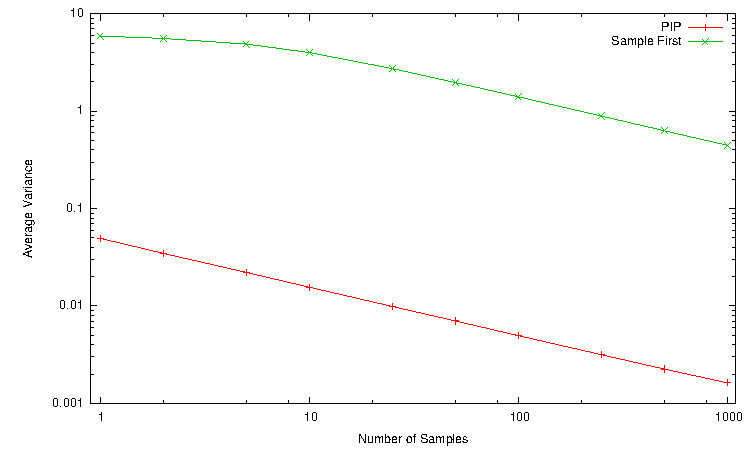
\includegraphics{graphics/variance.pdf}} \label{subfig:variance1}}
\subtable[]{\resizebox{3in}{!}{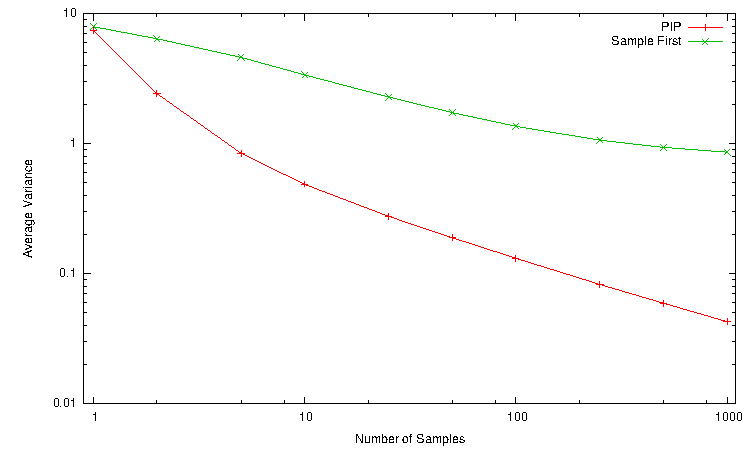
\includegraphics{graphics/variance2.pdf}}\label{subfig:variance2}}
%\begin{tabular}{cc}
%\resizebox{3in}{!}{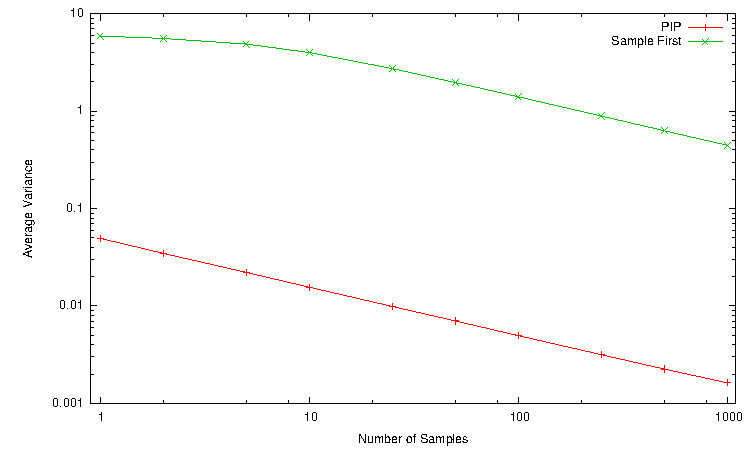
\includegraphics{graphics/variance.pdf}} &
%\resizebox{3in}{!}{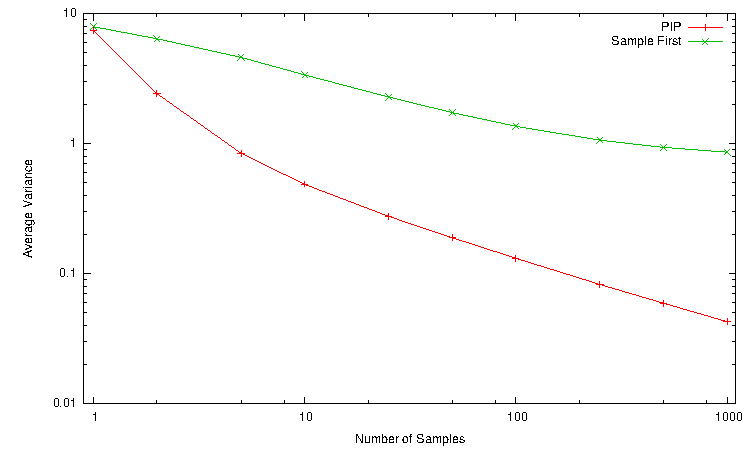
\includegraphics{graphics/variance2.pdf}} \\
%\textbf{(a)} & \textbf{(b)}
%\end{tabular}
\caption{Average variance across the results of 30 trials of (a) a simple group-by query with a selectivity of $0.005$, and (b) a complex selection query with an average selectivity of $0.05$.}
\label{fig:variance}
\end{center}
\end{figure*}

However, what the first three tests do not take into account is the accuracy of the results.  To illustrate this point, see Figure \ref{subfig:variance1}.  This figure shows the average normalized variance in the results of a query for predicted sales of 5000 parts in the database, given a Poisson distribution for the increase in sales and a popularity multiplier chosen from an exponential distribution.  As an additional restriction, the query considered only the extreme scenario where the given product had become extremely popular (resulting in a selectivity of $e^{-5.29} \approx 0.005$).  The variance was computed over 30 trials using the algebraically computed correct value as a mean, and then averaged over all 5000 parts.  Note that PIP's variance is over two orders of magnitude lower than the sample-first approach for a comparable number of samples.  This corresponds exactly to the selectivity of the query; as the query becomes more selective, the sample-first variance increases.  Furthermore, because CDF sampling is used to restrict the sampling bounds, the time taken by both approaches to compute an equivalent number of samples is equivalent.

A similar example is shown in Figure \ref{subfig:variance2}.  Here, a model is constructed for how much product suppliers are likely to be able to produce in the coming year based on an Exponential distribution, and for how much product the company expects to sell in the coming year as in Q1.  From this model, the expected underproduction is computed, with a lower bound of 0; the selection criterion considers only those worlds where demand exceeds supply.  For the purposes of this test, the model was chosen to generate an average selectivity of 0.05.  Though the comparison of 2 random variables necessitates the use of rejection sampling and increases the time PIP spends generating samples, the decision to drop a sample is made immediately after generating it; PIP can continue generating samples until it has a sufficient number, while the Sample-First approach must rerun the entire query.

Returning to Figure \ref{fig:querytimings}, the final timing test combines a simplified version of the prior two queries to simulate a risk management query that might be evaluated daily.  Given per-customer revenue forecasts, estimates for product manufacturing and shipping times, customer satisfaction thresholds, compute the expected revenue lost to customers dissatisfied with today's service.  For added realism, this query uses a precomputed table of part production and shipping times (which changes rarely enough that it can be updated monthly).  %This query is shown in Figure \ref{fig:timingq4}.

This query includes two distinct, independent sampling components: the expectation of revenue from a customer, and the probability that a customer will be dissatisfied.  A studious user may note this fact and hand optimize the query to compute these values independently.  However, without this optimization, a sample-first approach will generate one pair of values for each customer for each world.  As shown in the variance example, an arbitrarily large number of customer revenue values will be discarded and the query result will suffer.  In this test, customer satisfaction thresholds were set such that an average of 10\% of customers were dissatisfied.  Consequently sample-first discarded an average of 10\% of its values.  To maintain comparable accuracies, the sample-first query was evaluated with 10,000 samples while the PIP query remained at 1000 samples. 

We expand on this datapoint in Figure \ref{fig:scaling_selectivity} where we time the query used in Figure \ref{subfig:variance1} for varying selectivities.  The sample-first tests are run with $\frac{1}{selectivity}$ times as many samples as PIP to compensate for the lower variance.  Note that selectivity is a factor that a user must be aware of when constructing a query with sample-first while PIP is able to account for selectivity automatically, even if rejection sampling is required.

\begin{figure}
\begin{center}
\resizebox{3in}{!}{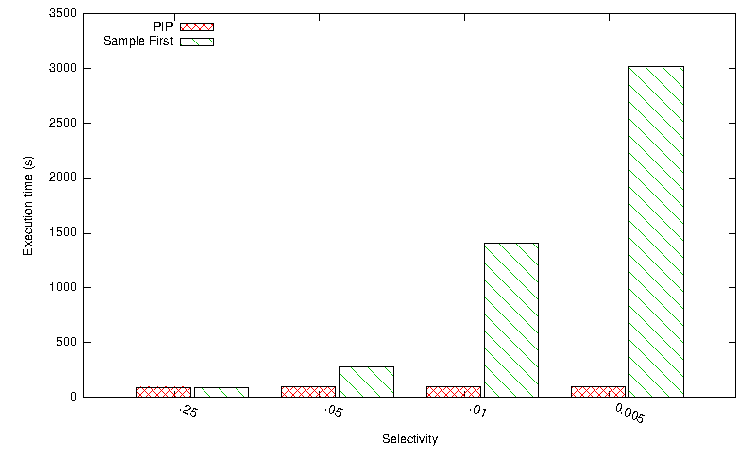
\includegraphics{graphics/scaling_selectivity.pdf}}
\caption{Time to complete a 1000 sample query, accounting for selectivity-induced loss of accuracy.}
\label{fig:scaling_selectivity}
\end{center}
\end{figure}

%\begin{figure}
%\begin{center}
%\resizebox{3in}{!}{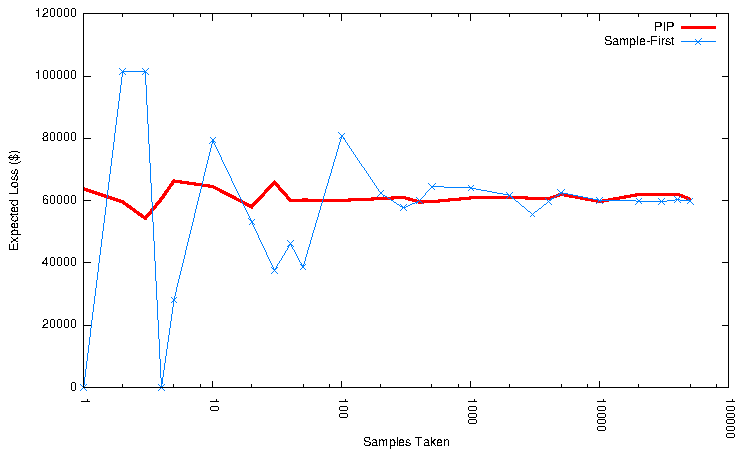
\includegraphics{graphics/iterative_refinement.pdf}}
%\caption{Variance as a function of samples in PIP and Sample-First.  Each data point is an estimate generated by a single run at the indicated number of samples}
%\label{fig:iterativerefinement}
%\end{center}
%\end{figure}
%
%
%Figure \ref{fig:iterativerefinement} demonstrates one extreme case of this in a comparison between Karp-Luby estimates and Sample-First estimates.  The results shown are for repeated executions of a query similar to query 4, save with a filter that removes all but approximately 10 clients.  In queries that do not involve a large linear aggregate, the sample-first approach disqualifies a sufficient number of possible worlds that subsequent expectation computations falter.  Conversely the Karp-Luby estimator has sufficient information that it can employ a precomputed CDF lookup table to compute each row's bag probabilities.  Because of this and the fact that it generates more ``useful'' samples, its results have a much lower variance with far fewer samples required.

%\begin{figure}[t!]
%%\footnotesize
%\begin{footnotesize}
%\begin{verbatim}
%create table `shipping_params' as
%  select 
%    avg   (l_shipdate    - o_orderdate) as ship_mu,
%    avg   (l_receiptdate - l_shipdate ) as arrv_mu,
%    stddev(l_shipdate    - o_orderdate) as ship_sigma,
%    stddev(l_receiptdate - l_shipdate ) as arrv_sigma,
%    l_partkey as p_partkey
%  from orders,lineitem
%  where o_orderkey = l_orderkey
%  group by partkey;
%alter table params add constraint "p_partkey_pkey" 
%  primary key (p_partkey);
%-- BEGIN TIMING QUERY --
%create temporary table q4_shipping as
%  select o_orderkey AS orderkey, o_custkey AS custkey,
%    CREATE VARIABLE(`Normal',ship_mu,ship_sigma)
%    CREATE VARIABLE(`Normal',arrv_mu,arrv_sigma)
%  from  orders,lineitem,shipping_params
%  where p_partkey = l_partkey;
%   and  o_orderdate = today()
%   and  o_orderkey  = l_orderkey;
%create temporary table q4_annoyed as
%  select custkey from q4_shipping where ship > 120
%union all
%  select custkey from q4_shipping where arrv > 90;
%create temporary table q4_order_increase as
%  select o_orderkey, o_custkey,
%     CREATE VARIABLE(`Poisson', increase) *
%       l_extended_price * (1.0 - l_discount) as rev
%  from (select newc / oldc as increase, custkey 
%    from (select o_custkey as custkey, 
%             sum(o_orderdate.year-1996.0) AS newc,
%             sum(1997.0-o_orderdate.year) AS oldc
%      where o_orderdate.year = 1997 
%        or  o_orderdate.year = 1996
%      group by custkey
%     ) as counts
%   ) as increase_per_cust,
%    orders
%  where custkey = o_custkey
% ) as var_increase_per_customer,
% (select lineitem.*,
%  from  nation,supplier, lineitem, partsupp
%  where n_name = 'japan' and n_nationkey = s_nationkey
%   and  s_suppkey = ps_suppkey
%   and  ps_partkey = l_partkey
%   and  ps_suppkey = l_suppkey
% ) as items_from_japan;
%-- BEGIN TIMING SAMPLE --
%select avg(confidence),
%       expected_sum_naive(rev, q4_annoyed)
%from   q4_annoyed,
%       (select o_custkey as custkey, rev
%        from   q4_revenue_gains
%       ) as revenues
%where  revenues.custkey = q4_annoyed.custkey;
%\end{verbatim}
%\end{footnotesize}
%
%\vspace{-5mm}
%
%\caption{Timing Query 4}
%\label{fig:timingq4}
%\end{figure}